\documentclass[tikz,border=6pt]{standalone}
\usepackage{pgfplots}
\pgfplotsset{compat=1.18}
\begin{document}
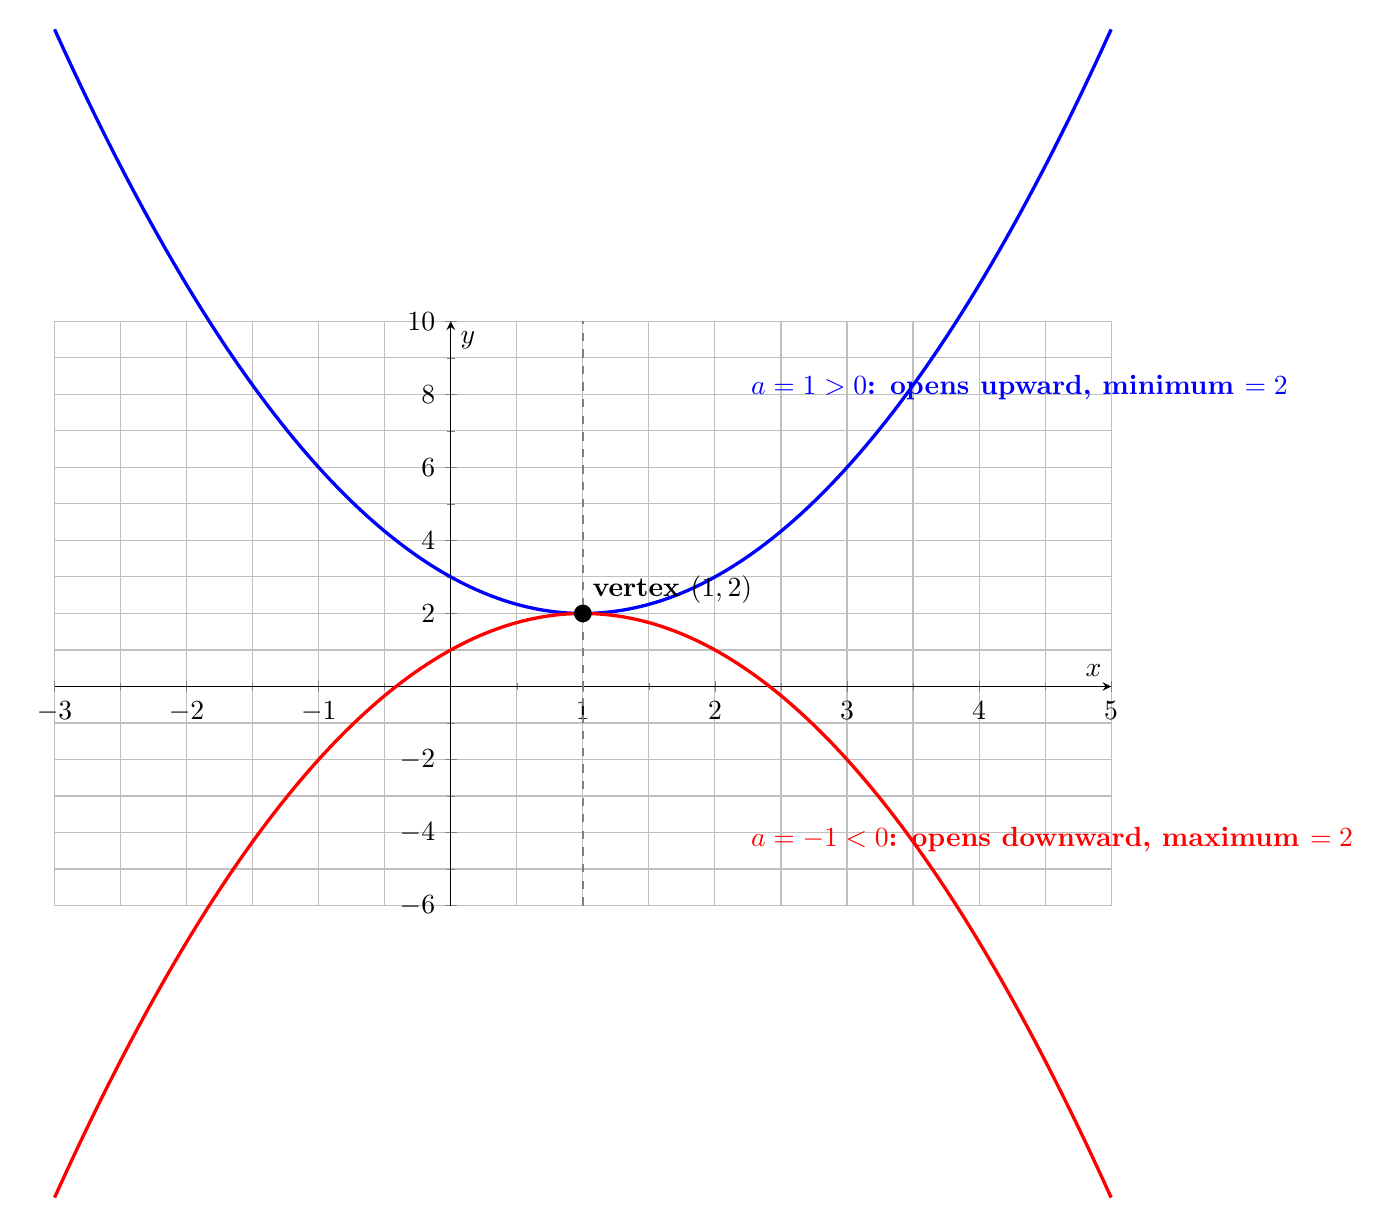
\begin{tikzpicture}
\begin{axis}[
  width=15cm,height=9cm,
  xmin=-3,xmax=5,ymin=-6,ymax=10,
  axis lines=middle,
  xlabel={$x$},ylabel={$y$},
  grid=both,minor tick num=1,
  samples=240,clip=false
]
\addplot[blue,very thick,domain=-3:5]{(x-1)^2+2};
\addplot[red,very thick,domain=-3:5]{-(x-1)^2+2};
\addplot[gray,dashed,thick] coordinates {(1,-6) (1,10)};
\addplot[black,only marks,mark=*,mark size=3pt] coordinates {(1,2)};
\node[black,font=\bfseries,anchor=south west] at (axis cs:1,2) {vertex $(1,2)$};
\node[blue,font=\bfseries,anchor=west] at (axis cs:2.2,8.2)
{$a=1>0$: opens upward, minimum $=2$};
\node[red,font=\bfseries,anchor=west] at (axis cs:2.2,-4.2)
{$a=-1<0$: opens downward, maximum $=2$};
\end{axis}
\end{tikzpicture}
\end{document}
